\section{Evaluation}
Recommendation quality is quantified with top-$K$ ranking metrics that emphasize slate relevance. We report precision@10, recall@10, and NDCG@10, computed as
\begin{align}
    \mathrm{P@K} &= \frac{1}{|U|} \sum_u \frac{|R_u \cap G_u|}{K}, \\
    \mathrm{R@K} &= \frac{1}{|U|} \sum_u \frac{|R_u \cap G_u|}{|G_u|}, \\
    \mathrm{DCG@K}(u) &= \sum_{j=1}^K \frac{\mathbf{1}[i_j \in G_u]}{\log_2(j+1)}, \\
    \mathrm{NDCG@K} &= \frac{1}{|U|} \sum_u \frac{\mathrm{DCG@K}(u)}{\mathrm{IDCG@K}(u)}.
\end{align}
Table~\ref{tab:metrics} summarizes current validation results and the hyperparameters selected for deployment, while Figure~\ref{fig:rank-eval-scatter} contextualizes how interaction frequency correlates with mean ratings.

\begin{table}[h]
    \centering
    \captionsetup{width=.9\linewidth}
    \caption{Ranking quality metrics and ALS hyperparameters.}
    \label{tab:metrics}
    \IfFileExists{auto/metrics_table.tex}{% Auto-generated metrics table (fallback)
\begin{tabular}{ll}
\toprule
Metric & Value \
\midrule
P@10 & N/A \
R@10 & N/A \
NDCG@10 & N/A \
Rank & N/A \
Reg & N/A \
Alpha & N/A \
Iters & N/A \
\bottomrule
\end{tabular}
}{\begin{tabular}{ll}\toprule Metric & Value \\ \midrule N/A & N/A \\ \bottomrule \end{tabular}}
\end{table}

\begin{figure}[h]
    \centering
    \IfFileExists{rating_vs_count_scatter.png}{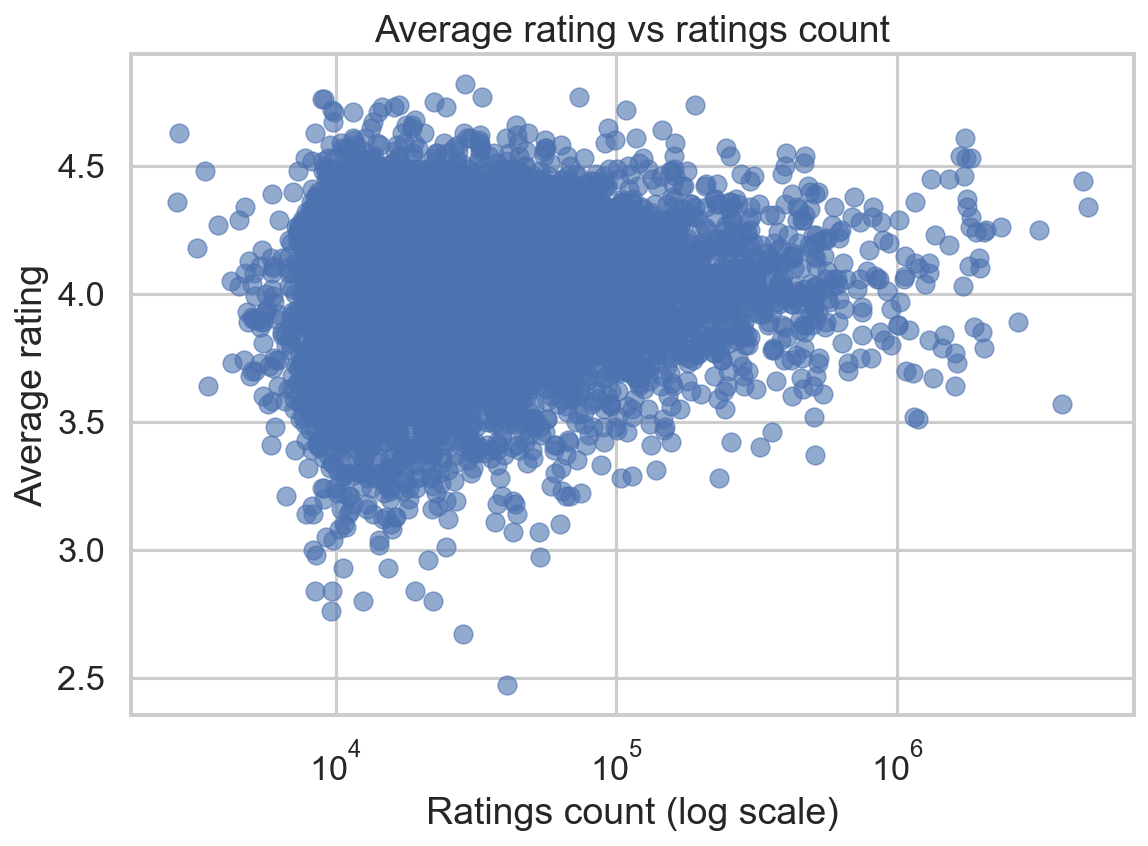
\includegraphics[width=.8\linewidth]{rating_vs_count_scatter.png}}{\begin{center}\textit{rating\_vs\_count\_scatter.png was unavailable at build time.}\end{center}}
    \caption{Items with more implicit feedback tend to stabilize toward middling ratings, informing ALS confidence weighting.}
    \label{fig:rank-eval-scatter}
\end{figure}

\metricsStatusNote
